\documentclass[journal]{IEEEtran}

% ---------------------------------------------------------------
% Packages
% ---------------------------------------------------------------
\usepackage{cite}
\usepackage{amsmath,amssymb,amsfonts}
\usepackage{graphicx}
\usepackage{textcomp}
\usepackage{xcolor}
\usepackage{booktabs}
\usepackage{multirow}
\usepackage{array}
\usepackage{url}
\usepackage{hyperref}
\usepackage{float}
\usepackage{placeins}

\graphicspath{{figures/}}

% ---------------------------------------------------------------
% Document
% ---------------------------------------------------------------
\begin{document}

\title{Evaluating Predictive Utility of Synthetic Liver Cirrhosis Data in IoMT: A Comparative Study of GAN, CTGAN, and TVAE with Consensus-Based Quality Filtering}

\author{\IEEEauthorblockN{Michael~Udousoro,~MSc~and~Mohammad~Farhan~Khan,~\IEEEmembership{PhD, Senior Lecturer}}
\IEEEauthorblockA{\textit{Department of Computer Science}\\
\textit{University of Roehampton}\\
London, United Kingdom}
\thanks{Manuscript received 2026.}}

\maketitle

% ---------------------------------------------------------------
% Abstract
% ---------------------------------------------------------------
\begin{abstract}
Expanding rare clinical datasets for Internet of Medical Things (IoMT) applications is constrained by patient privacy regulations and disease rarity. Most existing work evaluates synthetic data through distributional similarity metrics without directly testing whether augmentation improves prediction on real patients. This paper investigates that question using the Mayo Clinic Primary Biliary Cirrhosis (PBC) dataset, which yields 276 complete records after removing incomplete cases from 418 patients. Three generative architectures are trained from scratch in TensorFlow 2.15: a Vanilla GAN, a Conditional Tabular GAN (CTGAN), and a Tabular Variational Autoencoder (TVAE). Generated records pass through an IQR-based physiological plausibility filter, followed by a multi-method consensus voting procedure that retains only records independently corroborated by all three models. Distributional fidelity is assessed through tabular Fr\'{e}chet Inception Distance (FID), Kolmogorov-Smirnov tests, Jensen-Shannon divergence, Cohen's $d$, and chi-square tests; privacy risk is quantified via nearest-neighbour distance analysis. Predictive utility is evaluated by training Random Forest, Gradient Boosting, and Logistic Regression classifiers under four augmentation scenarios (real-only baseline, real + filtered CTGAN, real + consensus, and real + SMOTE) and testing exclusively on 83 held-out real patients, with 5-fold stratified cross-validation, 1000-resample bootstrap confidence intervals, and McNemar's exact test. CTGAN achieves the best distributional fidelity at FID 0.0751 (near-duplicate rate 9.0\%). No augmentation scenario produces a statistically significant improvement in held-out performance (all McNemar $p > 0.05$), confirming that distributional similarity does not guarantee predictive gain on real patients. However, consensus augmentation reduces Gradient Boosting cross-validation AUC variance 4.9-fold ($0.069 \rightarrow 0.014$) and Random Forest variance 3.4-fold ($0.053 \rightarrow 0.016$), demonstrating that cross-model agreement selects synthetic records that stabilise classifiers across training subsets. This stability benefit is directly relevant for reliable clinical decision support in IoMT deployments where consistent performance across patient subpopulations is critical.
\end{abstract}

\begin{IEEEkeywords}
Synthetic data generation, generative adversarial networks, variational autoencoder, liver cirrhosis, Internet of Medical Things, predictive utility, consensus voting, IQR filtering, patient privacy.
\end{IEEEkeywords}

% ---------------------------------------------------------------
% Section I: Introduction
% ---------------------------------------------------------------
\FloatBarrier
\section{Introduction}

The Internet of Medical Things has transformed how clinical biomarkers are collected, enabling continuous monitoring of liver enzymes, bilirubin concentrations, and albumin levels from wearable and implanted devices that feed directly into clinical decision support systems \cite{guo2021}, \cite{obeid2023}. As these systems grow more sophisticated, the demand for large, well-annotated patient datasets to train predictive models grows alongside them. The tension between that demand and the reality of clinical data availability is one of the defining challenges in medical machine learning. Privacy regulations, including GDPR and HIPAA, restrict what institutions can share, while rare conditions produce datasets that are inherently small. The Mayo Clinic Primary Biliary Cirrhosis trial is a concrete example: it enrolled 312 patients over more than a decade, and once records with incomplete measurements are removed, only 276 patients remain available for analysis \cite{kanwal2020}. Training robust classifiers on a dataset of that size is genuinely difficult.

Synthetic data generation through generative artificial intelligence has emerged as the most principled response to this situation. Rather than sharing real patient records, researchers can generate synthetic patients that statistically resemble the real population while not corresponding to any individual, enabling collaborative research without breaching privacy \cite{goncalves2020}, \cite{gonzales2023}. Generative Adversarial Networks and Variational Autoencoders have demonstrated genuine promise across medical imaging, physiological time series, and tabular clinical records \cite{yan2022}, \cite{nikolentzos2023}, \cite{che2017}. The difficulty is that the field has developed a habit of evaluating synthetic data through distributional lenses, measuring how similar synthetic samples are to real ones using feature-level statistics and aggregate distance metrics such as Fr\'{e}chet Inception Distance or Jensen-Shannon divergence. These are sensible measures of generation quality, but they answer a different question from the one that matters most clinically. The relevant operational question is whether augmenting a training set with synthetic patients actually produces a model that predicts real patient outcomes more accurately. Whether distributional similarity translates into predictive utility has received far less systematic attention, particularly for small, rare tabular clinical datasets in IoMT settings \cite{kababji2023}, \cite{espinosa2023}.

This paper addresses that gap through a controlled experimental pipeline applied to the PBC complete-case dataset of 276 patients (193 training, 83 held-out test, stratified 70/30 split with seed 42). Three deep generative models are trained from scratch in TensorFlow 2.15: a Vanilla GAN, a Conditional Tabular GAN that conditions generation on the patient outcome label (deceased vs.\ censored/transplanted), and a Tabular Variational Autoencoder. Two pre-augmentation quality controls are then applied. The first is an IQR-based physiological plausibility filter that removes synthetic records containing biomarker values outside Tukey fence bounds computed from real training patients. The second is a multi-method consensus voting mechanism that identifies a high-confidence synthetic subset agreed upon independently by all three generative models, based on the premise that a synthetic patient produced in the same region of feature space by three structurally different architectures is more likely to reflect a genuine distributional pattern than one produced by any single model.

The contributions of this work are as follows. First, three deep generative architectures are compared for tabular liver cirrhosis data in an IoMT setting, all built from scratch, allowing a fair head-to-head assessment of adversarial and variational approaches on the same dataset. Second, an IQR-based plausibility filter and a multi-method consensus voting mechanism are introduced as pre-augmentation quality controls. Third, a predictive utility evaluation framework is applied that benchmarks each augmentation strategy against both a real-data baseline and an SMOTE oversampling baseline, using 5-fold cross-validation, bootstrap confidence intervals, and McNemar's exact test on a held-out real test set.

The paper proceeds as follows. Section~\ref{sec:related} reviews relevant literature. Section~\ref{sec:methodology} describes the dataset, generative architectures, filtering pipeline, and experimental design. Section~\ref{sec:results} presents results, and Section~\ref{sec:conclusion} concludes.

% ---------------------------------------------------------------
% Section II: Related Work
% ---------------------------------------------------------------
\FloatBarrier
\section{Related Work}
\label{sec:related}

\subsection{Synthetic Data Generation for Healthcare}

Synthetic data generation has attracted sustained research interest as a means of making healthcare datasets more widely available without compromising patient privacy \cite{goncalves2020}, \cite{gonzales2023}, \cite{guillaudeux2023}. Gon\c{c}alves et al.\ conducted a systematic review of generation and evaluation methods, establishing that downstream utility, meaning the capacity of synthetic data to substitute for real data in analytical tasks, deserves equal attention alongside privacy preservation \cite{goncalves2020}. Gonzales et al.\ surveyed clinical applications across oncology, cardiology, and infectious disease, identifying tabular electronic health records as the domain with the greatest unmet need for robust generation methods \cite{gonzales2023}.

Classical augmentation approaches have well-documented limitations in this context. SMOTE addresses class imbalance by interpolating between existing minority-class training points and cannot generate samples outside the convex hull of observed data \cite{kumari2024}, \cite{figueira2022}. Rule-based and parametric generators offer transparency but fail to capture the non-linear dependencies characterising clinical biomarker profiles. Deep generative models learn these dependencies directly from data and have become the dominant approach for tabular clinical synthesis \cite{yan2022}, \cite{nikolentzos2023}.

\subsection{GAN Architectures for Tabular Clinical Data}

Generative Adversarial Networks train a generator against a discriminator through adversarial feedback \cite{vega2020}. In clinical settings, Che et al.\ showed that GAN-augmented training data can improve risk prediction from electronic health records \cite{che2017}, and Choi et al.\ proposed medGAN for generating multi-label discrete patient records \cite{choi2017}. Standard GAN architectures are prone to mode collapse and training instability when applied to heterogeneous tabular data combining continuous biomarkers, binary indicators, and ordinal staging variables \cite{lenz2021}, \cite{espinosa2023}. The Conditional Tabular GAN addresses these limitations by conditioning both generator and discriminator on a class label, ensuring minority classes receive proportional representation \cite{vega2020}, \cite{sharma2024}. The Tabular Variational Autoencoder takes a complementary approach, optimising a probabilistic lower bound on the data likelihood. Its encoder maps patient records into a continuous latent space while its decoder reconstructs records from samples drawn from that distribution, generating new patients at inference time by sampling from a standard normal prior \cite{nikolentzos2023}.

\subsection{Synthetic Data for IoMT}

IoMT infrastructures produce continuous streams of physiological measurements that clinical decision support systems must process reliably, requiring large labelled training sets \cite{guo2021}, \cite{obeid2023}. Meidan et al.\ showed that GAN-generated data improved anomaly detection in IoMT systems \cite{meidan2018}. D'Amico et al.\ demonstrated that AI-generated synthetic cohorts can accelerate research in haematological conditions where real patient numbers are similarly limited \cite{damico2023}. Kim et al.\ showed that synthetic augmentation improves survival prediction in early-onset colorectal cancer, a rare-disease tabular setting structurally similar to PBC \cite{kim2024}. Tucker et al.\ established that high-fidelity synthetic patient data can substitute for real data in evaluating healthcare software, provided quality is rigorously assessed \cite{tucker2020}.

\subsection{From Distributional Fidelity to Predictive Utility}

The dominant evaluation framework measures how closely generated samples resemble real data through marginal distributions and aggregate distance metrics \cite{yan2022}, \cite{figueira2022}, \cite{dankar2022}. Espinosa and Figueira found only a weak correlation between distributional and utility metrics across a range of datasets \cite{espinosa2023}. Foraker et al.\ showed that analytical results from synthetic data do not reliably replicate real-data findings even when distributional similarity is high \cite{foraker2020}. Kababji et al.\ concluded that the ability to reproduce hazard ratios from real patient data is a more clinically meaningful benchmark than FID alone \cite{kababji2023}. Kaabachi et al.\ identified the absence of held-out real-patient evaluation as a critical and recurring gap in the medical synthetic data literature \cite{kaabachi2023}. The present work is designed specifically to fill that gap.

\subsection{Multi-Model Ensemble Strategies and the Positioning of This Work}

Jiang et al.\ proposed a multi-source data augmentation framework for industrial fault diagnosis in which several GAN models are trained independently, and their outputs are pooled through cooperative and competitive mechanisms \cite{jiang2023}. The consensus voting mechanism introduced here shares this intuition but departs from it in two important respects: three structurally distinct architectures are used rather than multiple instances of the same one, and acceptance requires cross-architecture agreement rather than simply pooling all outputs.

Within the IoMT domain, Pandey et al.\ introduced MF-CGAN, a multifeature conditional GAN published in this journal that generates synthetic network traffic and health metrics by conditioning on multiple concurrent variables \cite{pandey2025}. The present work complements MF-CGAN in the clinical direction: the data consists of continuous laboratory biomarkers, ordinal disease staging, and binary clinical indicators measured at a single visit. The evaluation criterion differs as well: classifiers are trained on augmented data and tested exclusively on real held-out patients. The consensus voting mechanism introduced here has no analogue in MF-CGAN, and the results reveal that its primary benefit is not improved peak accuracy but substantially reduced model variance across cross-validation folds.

% ---------------------------------------------------------------
% Section III: Methodology
% ---------------------------------------------------------------
\FloatBarrier
\section{Methodology}
\label{sec:methodology}

\subsection{Dataset and Preprocessing}

The dataset used in this study is the Mayo Clinic Primary Biliary Cirrhosis (PBC) trial obtained from the UCI Machine Learning Repository \cite{kanwal2020}. The raw file contains 418 patient records and 20 columns. The patient identifier column carries no clinical information and is discarded. The remaining 19 columns consist of 11 continuous laboratory measurements (N\_Days, Age, Bilirubin, Cholesterol, Albumin, Copper, Alk\_Phos, SGOT, Triglycerides, Platelets, and Prothrombin), five binary clinical indicators (Sex, Drug, Ascites, Hepatomegaly, and Spiders), two ordinal variables (Edema coded as 0~=~none, 1~=~slight/suspected, 2~=~confirmed; Stage coded 1--4), and the binary survival outcome Status (0~=~censored/transplanted, 1~=~deceased).

Patients 313--418 belong to an observational cohort missing between 9 and 10 laboratory measurements each. Rather than imputing values collected under fundamentally different protocols (which would introduce systematic bias), complete-case analysis is applied: any row containing at least one missing value is removed, yielding 276 complete patient records. Categorical columns are numerically encoded: Sex (Female~=~0, Male~=~1), Drug (Placebo~=~0, D-penicillamine~=~1), Ascites/Hepatomegaly/Spiders (No~=~0, Yes~=~1), and Status (censored/transplanted~=~0, deceased~=~1). All features are then scaled to $[0, 1]$ using a MinMaxScaler fitted exclusively on the training partition to prevent data leakage.

\begin{figure}[t]
  \centering
  
\includegraphics[width=\columnwidth]{eda_correlation_matrix.png}
  \caption{Pearson correlation matrix across all 276 complete cases. Bilirubin shows strong positive correlations with Copper ($r = 0.46$), SGOT ($r = 0.42$), Cholesterol ($r = 0.39$), and Prothrombin ($r = 0.33$), reflecting the interlinked nature of hepatic synthetic and excretory function in PBC. N\_Days is negatively correlated with Bilirubin ($r = -0.43$) and Copper ($r = -0.36$), consistent with more severe biochemical profiles being associated with shorter survival.}
  \label{fig:corrmatrix}
\end{figure}

The 276 records are divided into a training set of 193 patients and a held-out test set of 83 patients using stratified random splitting with seed 42, preserving class balance in both partitions (training: 115 survived/transplanted = 59.6\%, 78 deceased = 40.4\%). The overall pipeline is illustrated in Fig.~\ref{fig:pipeline}.

\begin{figure}[t]
  \centering
  
\includegraphics[width=\columnwidth]{fig9_pipeline_flowchart.png}
  \caption{End-to-end synthetic data pipeline. The raw 418-patient dataset passes through a complete-case filter and a preprocessing stage before the 193-patient training set feeds three parallel generative models. Each model's 500 generated records pass through an IQR plausibility filter before all three filtered pools enter the consensus voting stage.}
  \label{fig:pipeline}
\end{figure}

\subsection{Generative Model Architectures}

All three models are implemented from scratch in TensorFlow 2.15 without third-party synthetic data libraries. Each model receives the MinMax-scaled training data and produces samples in the same normalised $[0, 1]$ range, which are inverse-transformed to recover original clinical units after generation. Each model generates 500 synthetic records.

\textbf{Vanilla GAN.} The generator maps a 100-dimensional noise vector $\mathbf{z}$ drawn from a standard normal distribution through two dense hidden layers of 128 and 256 units with Leaky ReLU activations ($\alpha = 0.2$) and batch normalisation (momentum~$= 0.8$) to a sigmoid output of dimension 18. The discriminator maps each patient record through two dense layers of 256 and 128 units with Leaky ReLU activations and dropout ($p = 0.3$). Both networks use the Adam optimiser with learning rate $2 \times 10^{-4}$ and $\beta_1 = 0.5$ for 500 epochs at batch size 32. The adversarial objectives are:
\begin{align}
\mathcal{L}_D &= -\mathbb{E}[\log D(\mathbf{x})] - \mathbb{E}[\log(1 - D(G(\mathbf{z})))] \\
\mathcal{L}_G &= -\mathbb{E}[\log D(G(\mathbf{z}))]
\end{align}

\textbf{Conditional Tabular GAN (CTGAN).} The CTGAN extends the Vanilla GAN by conditioning both generator and discriminator on the patient outcome label $\mathbf{y}$, supplied as a two-dimensional one-hot vector. The generator receives the concatenation $[\mathbf{z} \| \mathbf{y}]$, and the discriminator receives $[\mathbf{x} \| \mathbf{y}]$. Training uses balanced mini-batches, drawing equal numbers of survivors and deceased patients at each step. Architecture and optimiser settings match the Vanilla GAN, with training for 300 epochs.

\textbf{Tabular Variational Autoencoder (TVAE).} The encoder maps each patient record through two dense layers of 128 and 64 units with ReLU activations to a mean vector $\boldsymbol{\mu}$ and log-variance vector $\log(\boldsymbol{\sigma}^2)$ of dimension 32. A latent sample is drawn using the reparameterisation trick:
\begin{equation}
\mathbf{z} = \boldsymbol{\mu} + \boldsymbol{\varepsilon} \cdot \exp(0.5 \cdot \log(\boldsymbol{\sigma}^2)),
\end{equation}
where $\boldsymbol{\varepsilon}$ is drawn from a standard normal. The decoder maps $\mathbf{z}$ through two dense layers of 64 and 128 units with ReLU activations to a sigmoid output of dimension 18. The training objective is the Evidence Lower Bound (ELBO):
\begin{equation}
\mathcal{L}_{\text{TVAE}} = \mathbb{E}\!\left[\|\mathbf{x} - \hat{\mathbf{x}}\|^2\right] + \beta \cdot D_{\text{KL}}\!\left(\mathcal{N}(\boldsymbol{\mu}, \boldsymbol{\sigma}^2) \,\|\, \mathcal{N}(\mathbf{0}, \mathbf{I})\right)
\end{equation}
with $\beta = 1.0$, Adam optimiser at learning rate $1 \times 10^{-3}$, batch size 32, and 300 training epochs.

\begin{figure}[t]
  \centering
  
\includegraphics[width=\columnwidth]{fig0_training_losses.png}
  \caption{Training loss curves for all three generative models. Left: Vanilla GAN generator and discriminator losses over 500 epochs. Centre: CTGAN losses over 300 epochs, showing a pronounced peak near epoch 30 followed by convergence. Right: TVAE total ELBO loss over 300 epochs, falling sharply from 0.15 to approximately 0.08 by epoch 50 and then remaining stable.}
  \label{fig:training}
\end{figure}

\subsection{IQR-Based Physiological Plausibility Filter}

A Tukey fence filter is applied independently to each model's output. For each of the 11 continuous clinical features, the first and third quartiles, $Q_1$ and $Q_3$, are computed from the real training set alone. A synthetic record is retained only if every continuous feature value falls within $[Q_1 - 1.5 \times \text{IQR},\; Q_3 + 1.5 \times \text{IQR}]$. A single out-of-range value disqualifies the entire record. Binary and ordinal features are exempt because they are snapped to valid integer ranges during post-processing.

Applied to 500 generated records per model, the filter retained 226 GAN records (45.2\%), 210 CTGAN records (42.0\%), and all 500 TVAE records (100.0\%).

\begin{figure}[t]
  \centering
  
\includegraphics[width=\columnwidth]{fig2_iqr_filtering.png}
  \caption{Effect of IQR-based Tukey fence filtering on the Bilirubin distribution for all three generative models. Grey bars show real patient density. Pink bars show unfiltered synthetic distribution; coloured bars show the post-filter distribution. The GAN and CTGAN produce records extending beyond 15~mg/dL that the filter removes. The TVAE retains all generated records but produces a distribution shifted rightward relative to real patients.}
  \label{fig:iqr}
\end{figure}

\subsection{Multi-Method Consensus Voting}

A consensus voting mechanism is applied that retains only records independently corroborated by all three generative models. This approach is related to the multi-source data augmentation strategy of Jiang et al.\ \cite{jiang2023}, who combine outputs from multiple independently trained GANs to reduce distribution skewness. The present work differs in that three structurally distinct architectures are used, and acceptance requires cross-architecture agreement rather than simply pooling all outputs.

A StandardScaler is fitted on the union of all three filtered datasets. For each candidate record from one model, the minimum Euclidean distance to any record from each of the other two models is computed in standardised space. The candidate is accepted if both other models have a record within tolerance~$= 5.0$ standardised units. This process repeats with each filtered dataset as the candidate pool in turn, and exact duplicates are removed from the final set. The threshold of 5.0 was selected on the basis of a systematic sensitivity analysis conducted across eight values from 2.5 to 6.0. At thresholds below 4.5, the accepted set contains fewer than 13\% deceased patients, introducing a severe class imbalance relative to the real training cohort (40\% deceased). At 5.0, class balance recovers to 15.3\% and the FID score reaches 0.1116, after which further increases in threshold yield only marginal FID improvements (0.1027 at 5.5, 0.0956 at 6.0) while adding records with progressively weaker cross-model agreement. The value of 5.0 therefore represents the point at which class balance becomes acceptable and the quality improvement curve begins to flatten. To address the pool-size imbalance across the three filtered datasets (GAN 226 records, CTGAN 210 records, TVAE 500 records), the TVAE pool is randomly downsampled to 210 records before voting, matching the size of the smallest adversarial pool. This equalisation reduces TVAE's contribution from 61.9\% to 37.7\% while CTGAN rises to 32.8\% and GAN rises to 29.5\%, giving the two higher-fidelity adversarial models a proportionally stronger role in the consensus. The equalised consensus of 555 records achieves FID 0.0862, compared to 0.1116 without equalisation, and reduces the near-duplicate rate from 28.4\% to 0.4\%, substantially improving the privacy safety profile of the consensus set.

\begin{figure}[t]
  \centering
  
\includegraphics[width=\columnwidth]{fig5_consensus_distribution.png}
  \caption{Source composition of the 555 equalised consensus records. Left: absolute record counts per generative method after consensus voting with TVAE pool downsampled to 210. Right: proportional contribution as a pie chart. GAN contributes 29.5\%, CTGAN 32.8\%, and TVAE 37.7\%.}
  \label{fig:consensus}
\end{figure}

\subsection{Synthetic Data Quality Evaluation}

Distributional fidelity is assessed using a tabular proxy Fr\'{e}chet Inception Distance computed on the 18-dimensional feature vectors:
\begin{equation}
\text{FID} = \|\boldsymbol{\mu}_r - \boldsymbol{\mu}_s\|^2 + \text{Tr}\!\left(\boldsymbol{\Sigma}_r + \boldsymbol{\Sigma}_s - 2(\boldsymbol{\Sigma}_r \boldsymbol{\Sigma}_s)^{1/2}\right).
\end{equation}
Lower values indicate greater distributional alignment. Per-feature Kolmogorov-Smirnov tests, Jensen-Shannon divergence, Cohen's $d$, Shapiro-Wilk normality tests, and chi-square tests for categorical features provide a granular distributional profile. Privacy risk is assessed through nearest-neighbour distance analysis. For each synthetic record, the Euclidean distance to the closest real training patient is computed in StandardScaler-normalised feature space across all 18 input features. A record is flagged as a near-duplicate if its distance falls below the 5th percentile of real-to-real nearest-neighbour distances, a data-driven threshold that identifies synthetic records closer to any real patient than 95\% of real patients are to their nearest real neighbour.

\subsection{Predictive Utility Evaluation}

Predictive utility is evaluated by training Random Forest (RF), Gradient Boosting (GB), and Logistic Regression (LR) classifiers under four training scenarios and testing on the 83-patient held-out real test set:
\begin{itemize}
  \item \textbf{Scenario A:} 193 real patients only (baseline).
  \item \textbf{Scenario B:} 193 real + 210 IQR-filtered CTGAN records (403 total). CTGAN is selected here because it achieves the lowest FID among individual methods.
  \item \textbf{Scenario C:} 193 real + 555 consensus records (748 total).
  \item \textbf{Scenario D:} 193 real patients augmented with SMOTE oversampling (classical baseline).
\end{itemize}
All classifiers use default scikit-learn hyperparameters. Evaluation metrics are Accuracy, F1, Precision, Recall, and AUC-ROC. 5-fold stratified cross-validation, 1000-resample bootstrap confidence intervals, and McNemar's exact test complement the single-split evaluation. All random seeds are fixed at 42.

% ---------------------------------------------------------------
% Section IV: Results and Discussion
% ---------------------------------------------------------------
\FloatBarrier
\section{Results and Discussion}
\label{sec:results}

\subsection{Synthetic Data Retention and IQR Filtering}

Table~\ref{tab:retention} summarises IQR filter retention rates and FID scores. The GAN and CTGAN each reject more than half of their generated records; the TVAE retains all 500. The consensus procedure accepts 555 records from the equalised filtered pools (TVAE downsampled to 210).

\begin{table}[!t]
  \centering
  \caption{Synthetic Data Retention and FID Scores}
  \label{tab:retention}
  \begin{tabular}{lcccc}
    \toprule
    Method & Generated & Retained & Retention & FID \\
    \midrule
    Vanilla GAN   & 500 & 226 & 45.2\% & 0.0972 \\
    CTGAN         & 500 & 210 & 42.0\% & 0.0751 \\
    TVAE          & 500 & 500 & 100.0\% & 0.2194 \\
    Consensus     & ---  & 555 & ---   & 0.0862 \\
    \bottomrule
  \end{tabular}
\end{table}

\subsection{Distributional Fidelity}

Fig.~\ref{fig:fid} shows the tabular FID scores for all four synthetic datasets. CTGAN achieves the lowest FID of 0.0751, followed by the Vanilla GAN at 0.0972. The TVAE produces an FID of 0.2194 despite retaining all generated records, confirming that smooth variational generation reduces distributional sharpness. The equalised consensus set scores 0.0862.

\begin{figure}[t]
  \centering
  
\includegraphics[width=\columnwidth]{fig1_fid_comparison.png}
  \caption{Tabular Fr\'{e}chet Inception Distance scores for all four synthetic datasets. Lower scores indicate greater distributional alignment with real training data. CTGAN achieves the lowest FID at 0.0751. The TVAE, despite retaining all 500 generated records through the IQR filter, shows the highest FID at 0.2194, reflecting over-smoothing of clinical feature distributions. The equalised consensus set scores 0.0862, below the individual TVAE FID, confirming that pool equalisation improves distributional fidelity by reducing over-representation of variational samples.}
  \label{fig:fid}
\end{figure}

Fig.~\ref{fig:distributions} compares feature distributions for six representative clinical variables. Albumin and Prothrombin are well reproduced by GAN and CTGAN. Bilirubin is the most challenging feature: the TVAE distribution is noticeably shifted rightward relative to real patients, while GAN and CTGAN align better with the concentrated low-value peak.

\begin{figure}[t]
  \centering
  
\includegraphics[width=\columnwidth]{fig3_distribution_comparison.png}
  \caption{Feature distribution comparison between real training data and all four synthetic methods for six representative clinical variables: Bilirubin, Albumin, Prothrombin, Cholesterol, Copper, and SGOT. GAN and CTGAN reproduce Albumin and Prothrombin closely, while all methods show distributional divergence on the heavily right-skewed Bilirubin and Cholesterol features.}
  \label{fig:distributions}
\end{figure}

Fig.~\ref{fig:corrcomparison} compares the Pearson correlation structure of real patient data against the consensus synthetic dataset. The consensus set preserves the dominant pairwise associations, including the strong positive Bilirubin-Copper relationship and the negative N\_Days-Bilirubin association.

\begin{figure}[t]
  \centering
  
\includegraphics[width=\columnwidth]{fig4_correlation_heatmap.png}
  \caption{Pearson correlation structure comparison between real patient data (left) and consensus synthetic data (right). The consensus set preserves the dominant clinical associations, including the strong positive Bilirubin-Copper relationship ($r = 0.46$ in real data) and the negative N\_Days-Bilirubin association ($r = -0.43$), though weaker correlations are attenuated.}
  \label{fig:corrcomparison}
\end{figure}

Fig.~\ref{fig:tsne} shows the t-SNE projection of real patients and each synthetic method into two dimensions. The GAN and CTGAN filtered sets mix reasonably with the real patient manifold. The TVAE points spread more widely, with portions falling outside the real patient contours. The consensus set fills the central high-density region, confirming that cross-model agreement selects records from the most representative zone of feature space.

\begin{figure}[t]
  \centering
  
\includegraphics[width=\columnwidth]{tsne_real_vs_synthetic.png}
  \caption{t-SNE two-dimensional projection of real patients and each synthetic method in the original 18-dimensional feature space. GAN and CTGAN filtered sets show reasonable overlap with the real patient manifold. TVAE points spread more widely, with portions falling outside the real patient density contours. The consensus set fills the central high-density region.}
  \label{fig:tsne}
\end{figure}

Per-feature KS tests reveal a consistent pattern. The filtered GAN shows no significant distributional difference from real training data on N\_Days (KS~$= 0.095$, $p = 0.282$), Age (KS~$= 0.067$, $p = 0.707$), and Albumin (KS~$= 0.116$, $p = 0.111$), but diverges significantly on Bilirubin (KS~$= 0.468$), Alk\_Phos (KS~$= 0.688$), and SGOT (KS~$= 0.325$). The TVAE diverges significantly on all 11 continuous features. The consensus set achieves substantially smaller KS statistics on the most challenging biomarkers: Bilirubin KS~$= 0.164$ vs.\ GAN's 0.468; Alk\_Phos KS~$= 0.181$ vs.\ GAN's 0.688.

\subsection{Privacy Risk Assessment}

Fig.~\ref{fig:privacy} shows the privacy risk analysis using nearest-neighbour distances in standardised feature space. GAN and CTGAN distributions are centred well above the risk threshold (5th percentile of real-to-real distances), indicating that most adversarially generated records fall at a safe distance from any real patient. The TVAE and consensus distributions have substantial mass below the threshold, reflecting the broader coverage of the variational latent space and the cross-model acceptance criterion.

\begin{figure}[t]
  \centering
  
\includegraphics[width=\columnwidth]{privacy_risk_analysis.png}
  \caption{Privacy disclosure risk analysis using nearest-neighbour distances in standardised feature space. Left: violin plots of distances from each synthetic record to its closest real training patient. The red dashed line marks the risk threshold at the 5th percentile of real-to-real distances. GAN and CTGAN distributions are centred above this threshold. Right: near-duplicate rates by method. GAN (5.3\%) and CTGAN (9.0\%) present low privacy risk, while TVAE (38.2\%) and consensus (28.4\%) warrant caution in privacy-sensitive IoMT deployments.}
  \label{fig:privacy}
\end{figure}

\begin{table}[!t]
  \centering
  \caption{Privacy Risk Analysis}
  \label{tab:privacy}
  \begin{tabular}{lcccc}
    \toprule
    Method & Records & Mean Dist. & Near-Dup. & Rate \\
    \midrule
    GAN (filtered)   & 226 & 2.85 & 12  & 5.3\%  \\
    CTGAN (filtered) & 210 & 2.94 & 19  & 9.0\%  \\
    TVAE (filtered)  & 500 & 3.12 & 191 & 38.2\% \\
    Consensus        & 555 & $\sim$1.9  & 2   & 0.4\%  \\
    \bottomrule
  \end{tabular}
\end{table}

\subsection{Predictive Utility on the Held-Out Test Set}

Table~\ref{tab:performance} reports complete test-set metrics across all four scenarios.

\begin{table*}[t]
  \centering
  \caption{Test-Set Classification Performance (83 Real Held-Out Patients)}
  \label{tab:performance}
  \begin{tabular}{llccccccc}
    \toprule
    Scenario & Classifier & $n_{\text{train}}$ & Accuracy & F1 & Precision & Recall & AUC \\
    \midrule
    A: Baseline       & Random Forest      & 193 & 0.7831 & 0.7848 & 0.7901 & 0.7831 & 0.8479 \\
    A: Baseline       & Gradient Boosting  & 193 & 0.7831 & 0.7852 & 0.7955 & 0.7831 & \textbf{0.8776} \\
    A: Baseline       & Logistic Regression& 193 & 0.7711 & 0.7735 & 0.7940 & 0.7711 & 0.8291 \\
    \midrule
    B: Real + CTGAN   & Random Forest      & 403 & 0.7590 & 0.7616 & 0.7782 & 0.7590 & 0.8418 \\
    B: Real + CTGAN   & Gradient Boosting  & 403 & 0.7590 & 0.7616 & 0.7782 & 0.7590 & 0.8721 \\
    B: Real + CTGAN   & Logistic Regression& 403 & 0.7590 & 0.7616 & 0.7782 & 0.7590 & 0.8455 \\
    \midrule
    C: Real + Consensus & Random Forest    & 748 & 0.7590 & 0.7609 & 0.7663 & 0.7590 & 0.8542 \\
    C: Real + Consensus & Gradient Boosting& 748 & 0.7831 & 0.7854 & 0.8022 & 0.7831 & 0.8503 \\
    C: Real + Consensus & Logistic Regression & 748 & 0.7831 & 0.7841 & 0.7860 & 0.7831 & 0.8491 \\
    \midrule
    D: Real + SMOTE   & Random Forest      & 230 & 0.7470 & 0.7496 & 0.7628 & 0.7470 & 0.8388 \\
    D: Real + SMOTE   & Gradient Boosting  & 230 & \textbf{0.8072} & \textbf{0.8087} & 0.8140 & 0.8072 & 0.8661 \\
    D: Real + SMOTE   & Logistic Regression& 230 & 0.7711 & 0.7735 & 0.7940 & 0.7711 & 0.8297 \\
    \bottomrule
  \end{tabular}
\end{table*}

Fig.~\ref{fig:roc} shows the ROC curves for all three classifiers across all four scenarios on the 83-patient real held-out test set. All curves lie substantially above the random classifier diagonal. Gradient Boosting under Scenario A achieves the highest AUC at 0.878, while Logistic Regression under Scenario C achieves the highest AUC gain from augmentation at 0.855.

\begin{figure}[t]
  \centering
  
\includegraphics[width=\columnwidth]{roc_curves.png}
  \caption{ROC curves by classifier and training scenario on the 83-patient real held-out test set: Random Forest (left), Gradient Boosting (centre), Logistic Regression (right). All curves lie substantially above the random classifier diagonal. Gradient Boosting under Scenario A achieves the highest AUC at 0.878. Scenario D (SMOTE) achieves the highest overall accuracy at 0.807 under Gradient Boosting.}
  \label{fig:roc}
\end{figure}

Fig.~\ref{fig:prcurves} shows Precision-Recall curves across all four scenarios and classifiers. PR curves are particularly informative for this dataset given its class imbalance (78 deceased versus 115 survivors in the training set).

\begin{figure}[t]
  \centering
  
\includegraphics[width=\columnwidth]{pr_curves.png}
  \caption{Precision-Recall curves by classifier and training scenario on the 83-patient held-out test set. All classifiers maintain precision above 0.7 across a wide recall range. Gradient Boosting under Scenarios A and D achieve the highest average precision.}
  \label{fig:prcurves}
\end{figure}

Fig.~\ref{fig:auc} shows AUC scores across all three classifiers and all four scenarios. Every scenario and classifier combination exceeds AUC~$= 0.8$ comfortably, confirming that baseline real-data models are already clinically useful and that no augmentation strategy degrades discrimination below a clinically meaningful threshold.

\begin{figure}[t]
  \centering
  
\includegraphics[width=\columnwidth]{auc_detailed_comparison.png}
  \caption{AUC scores across all three classifiers and all four training scenarios (A through D). The green dashed reference line marks AUC~$= 0.8$ and the red dashed line marks AUC~$= 0.5$. All scenario-classifier combinations exceed 0.8 comfortably. Gradient Boosting under Scenario A achieves the highest AUC at 0.878.}
  \label{fig:auc}
\end{figure}

Fig.~\ref{fig:heatmap} presents the F1-score heatmap across all four scenarios. The highest F1 scores appear in Scenario A for Gradient Boosting and Random Forest at 0.785, and in Scenario D for Gradient Boosting at 0.809. Gradient Boosting is the only classifier whose F1 falls monotonically as synthetic augmentation volume increases (Scenario A to C).

\begin{figure}[t]
  \centering
  
\includegraphics[width=\columnwidth]{fig6_performance_heatmap.png}
  \caption{F1-score heatmap across all four scenarios (A through D) for all three classifiers. Darker blue indicates higher F1. Gradient Boosting under Scenario D achieves the highest F1 at 0.809. Under Scenario C, Gradient Boosting degrades to 0.738 while Logistic Regression and Random Forest hold at 0.773 and 0.784 respectively.}
  \label{fig:heatmap}
\end{figure}

Fig.~\ref{fig:modelcomp} presents a grouped bar comparison of accuracy, F1, and AUC across all four scenarios and classifiers, enabling a direct visual comparison between augmentation strategies and the real-data baseline. Fig.~\ref{fig:allmetrics} extends this view to all five evaluation metrics across scenarios.

\begin{figure}[t]
  \centering
  
\includegraphics[width=\columnwidth]{fig7_model_comparison.png}
  \caption{Grouped bar chart comparing classifier performance across all four training scenarios. No augmentation scenario uniformly outperforms the baseline across all classifiers and metrics.}
  \label{fig:modelcomp}
\end{figure}

\begin{figure}[t]
  \centering
  
\includegraphics[width=\columnwidth]{fig8_all_metrics.png}
  \caption{Line plot of all five evaluation metrics (Accuracy, F1, Precision, Recall, AUC) across the four training scenarios for each classifier. Trajectories are generally flat or slightly declining from Scenario A through Scenarios B and C, with Scenario D producing a modest accuracy gain for Gradient Boosting.}
  \label{fig:allmetrics}
\end{figure}

\subsection{Cross-Validation Stability}

Table~\ref{tab:cv} presents 5-fold stratified cross-validation AUC results. Consensus augmentation in Scenario C produces the highest mean CV AUC for both Random Forest (0.898) and Gradient Boosting (0.881). The standard deviation of CV AUC falls sharply: Gradient Boosting variance drops from 0.069 in Scenario A to 0.014 in Scenario C, a 4.9-fold reduction. Random Forest variance drops from 0.053 to 0.016, a 3.4-fold reduction.

\begin{table}[!t]
  \centering
  \caption{5-Fold Cross-Validation AUC (Mean $\pm$ Std)}
  \label{tab:cv}
  \begin{tabular}{lccc}
    \toprule
    Scenario & RF & GB & LR \\
    \midrule
    A: Baseline       & $0.878 \pm 0.053$ & $0.854 \pm 0.069$ & $0.805 \pm 0.047$ \\
    B: Real + CTGAN   & $0.891 \pm 0.028$ & $0.873 \pm 0.032$ & $0.867 \pm 0.034$ \\
    C: Real + Consensus & $\mathbf{0.898 \pm 0.016}$ & $\mathbf{0.881 \pm 0.014}$ & $0.832 \pm 0.025$ \\
    D: Real + SMOTE   & $0.886 \pm 0.045$ & $0.860 \pm 0.063$ & $0.852 \pm 0.052$ \\
    \bottomrule
  \end{tabular}
\end{table}

\subsection{Bootstrap Confidence Intervals and McNemar's Test}

Tables~\ref{tab:bootstrap} and~\ref{tab:mcnemar} report 95\% bootstrap confidence intervals for test-set AUC and McNemar's exact test results covering all four augmentation scenarios. All confidence intervals overlap substantially across scenarios, and all McNemar p-values exceed 0.28, confirming that no augmentation scenario produces a statistically significant change in predictive accuracy over the real-data baseline on the 83-patient held-out test set.

\begin{table}[!t]
  \centering
  \caption{95\% Bootstrap Confidence Intervals for Test-Set AUC (1000 resamples)}
  \label{tab:bootstrap}
  \begin{tabular}{llcc}
    \toprule
    Scenario & Classifier & AUC & 95\% CI \\
    \midrule
    A: Baseline       & RF  & 0.8479 & [0.754, 0.938] \\
    A: Baseline       & GB  & 0.8776 & [0.788, 0.948] \\
    A: Baseline       & LR  & 0.8291 & [0.728, 0.916] \\
    B: Real + CTGAN   & RF  & 0.8418 & [0.742, 0.934] \\
    B: Real + CTGAN   & GB  & 0.8721 & [0.776, 0.948] \\
    B: Real + CTGAN   & LR  & 0.8455 & [0.746, 0.934] \\
    C: Real + Consensus & RF & 0.8539 & [0.760, 0.933] \\
    C: Real + Consensus & GB & 0.8321 & [0.731, 0.919] \\
    C: Real + Consensus & LR & 0.8552 & [0.756, 0.935] \\
    D: Real + SMOTE   & RF  & 0.8388 & [0.742, 0.930] \\
    D: Real + SMOTE   & GB  & 0.8661 & [0.776, 0.946] \\
    D: Real + SMOTE   & LR  & 0.8297 & [0.729, 0.917] \\
    \bottomrule
  \end{tabular}
\end{table}

\begin{table}[!t]
  \centering
  \caption{McNemar's Exact Test (Augmented vs.\ Baseline, $\alpha = 0.05$)}
  \label{tab:mcnemar}
  \begin{tabular}{llccc}
    \toprule
    Classifier & Comparison & $n_{10}$ & $n_{01}$ & $p$-value \\
    \midrule
    Random Forest       & A vs.\ B & 3 & 1 & 0.625 \\
    Random Forest       & A vs.\ C & 2 & 2 & 1.000 \\
    Random Forest       & A vs.\ D & 4 & 4 & 1.000 \\
    Gradient Boosting   & A vs.\ B & 4 & 2 & 0.688 \\
    Gradient Boosting   & A vs.\ C & 6 & 2 & 0.289 \\
    Gradient Boosting   & A vs.\ D & 2 & 4 & 0.688 \\
    Logistic Regression & A vs.\ B & 2 & 1 & 1.000 \\
    Logistic Regression & A vs.\ C & 4 & 4 & 1.000 \\
    Logistic Regression & A vs.\ D & 0 & 0 & 1.000 \\
    \bottomrule
    \multicolumn{5}{l}{\footnotesize $n_{10}$: baseline correct, augmented wrong; $n_{01}$: augmented correct, baseline wrong.}
  \end{tabular}
\end{table}

\FloatBarrier
\subsection{Discussion}

The results offer a nuanced picture of what synthetic augmentation can and cannot achieve on a rare tabular clinical dataset in an IoMT context. On the held-out test set, no augmentation strategy produces a statistically significant improvement over training on real data alone. This is a meaningful finding rather than a failure: the 276-patient PBC dataset contains sufficient signal for Gradient Boosting to reach AUC~$= 0.878$ without any augmentation, and adding synthetic patients that are distributional approximations of the real data does not substantially change what classifiers learn about the survival decision boundary when evaluated on 83 real patients.

The cross-validation results reveal a genuine benefit that single-split evaluation obscures. Consensus augmentation reduces Gradient Boosting variance 4.9-fold and Random Forest variance 3.4-fold across folds, indicating that the additional synthetic patients stabilise classifiers across different subsets of the training data. In an IoMT deployment setting where a clinical decision support model must perform reliably across patients of different disease stages, ages, and treatment backgrounds, a model with lower cross-validation variance is more trustworthy than one that achieves peak performance on one partition by chance.

A post-hoc power analysis was conducted to characterise the statistical sensitivity of the McNemar test on 83 patients. Assuming a typical discordant pair rate of approximately 15 per cent (12 discordant pairs per comparison), the test has only 49\% power to detect a moderate effect in which the augmented model wins 70\% of discordant cases, corresponding to a true accuracy gain of approximately 5.8 percentage points. Bootstrap simulation over 1000 synthetic trials confirms that McNemar's test on 83 patients has only 9\% power to detect a genuine 5 percentage-point improvement in accuracy. Achieving 80\% power at that modest effect size would require approximately 300 held-out patients. Fig.~\ref{fig:power} shows the power curve across discordant pair counts and the required sample size as a function of true accuracy improvement. These results do not invalidate the null finding; the observed p-values ranged from 0.50 to 1.00, far above the 0.05 threshold, rather than clustering at values just above it. However, they establish that the study is underpowered for detecting small benefits, and that a replication on a larger cohort is necessary before augmentation can be conclusively ruled out as clinically beneficial.

\begin{figure}[t]
  \centering
  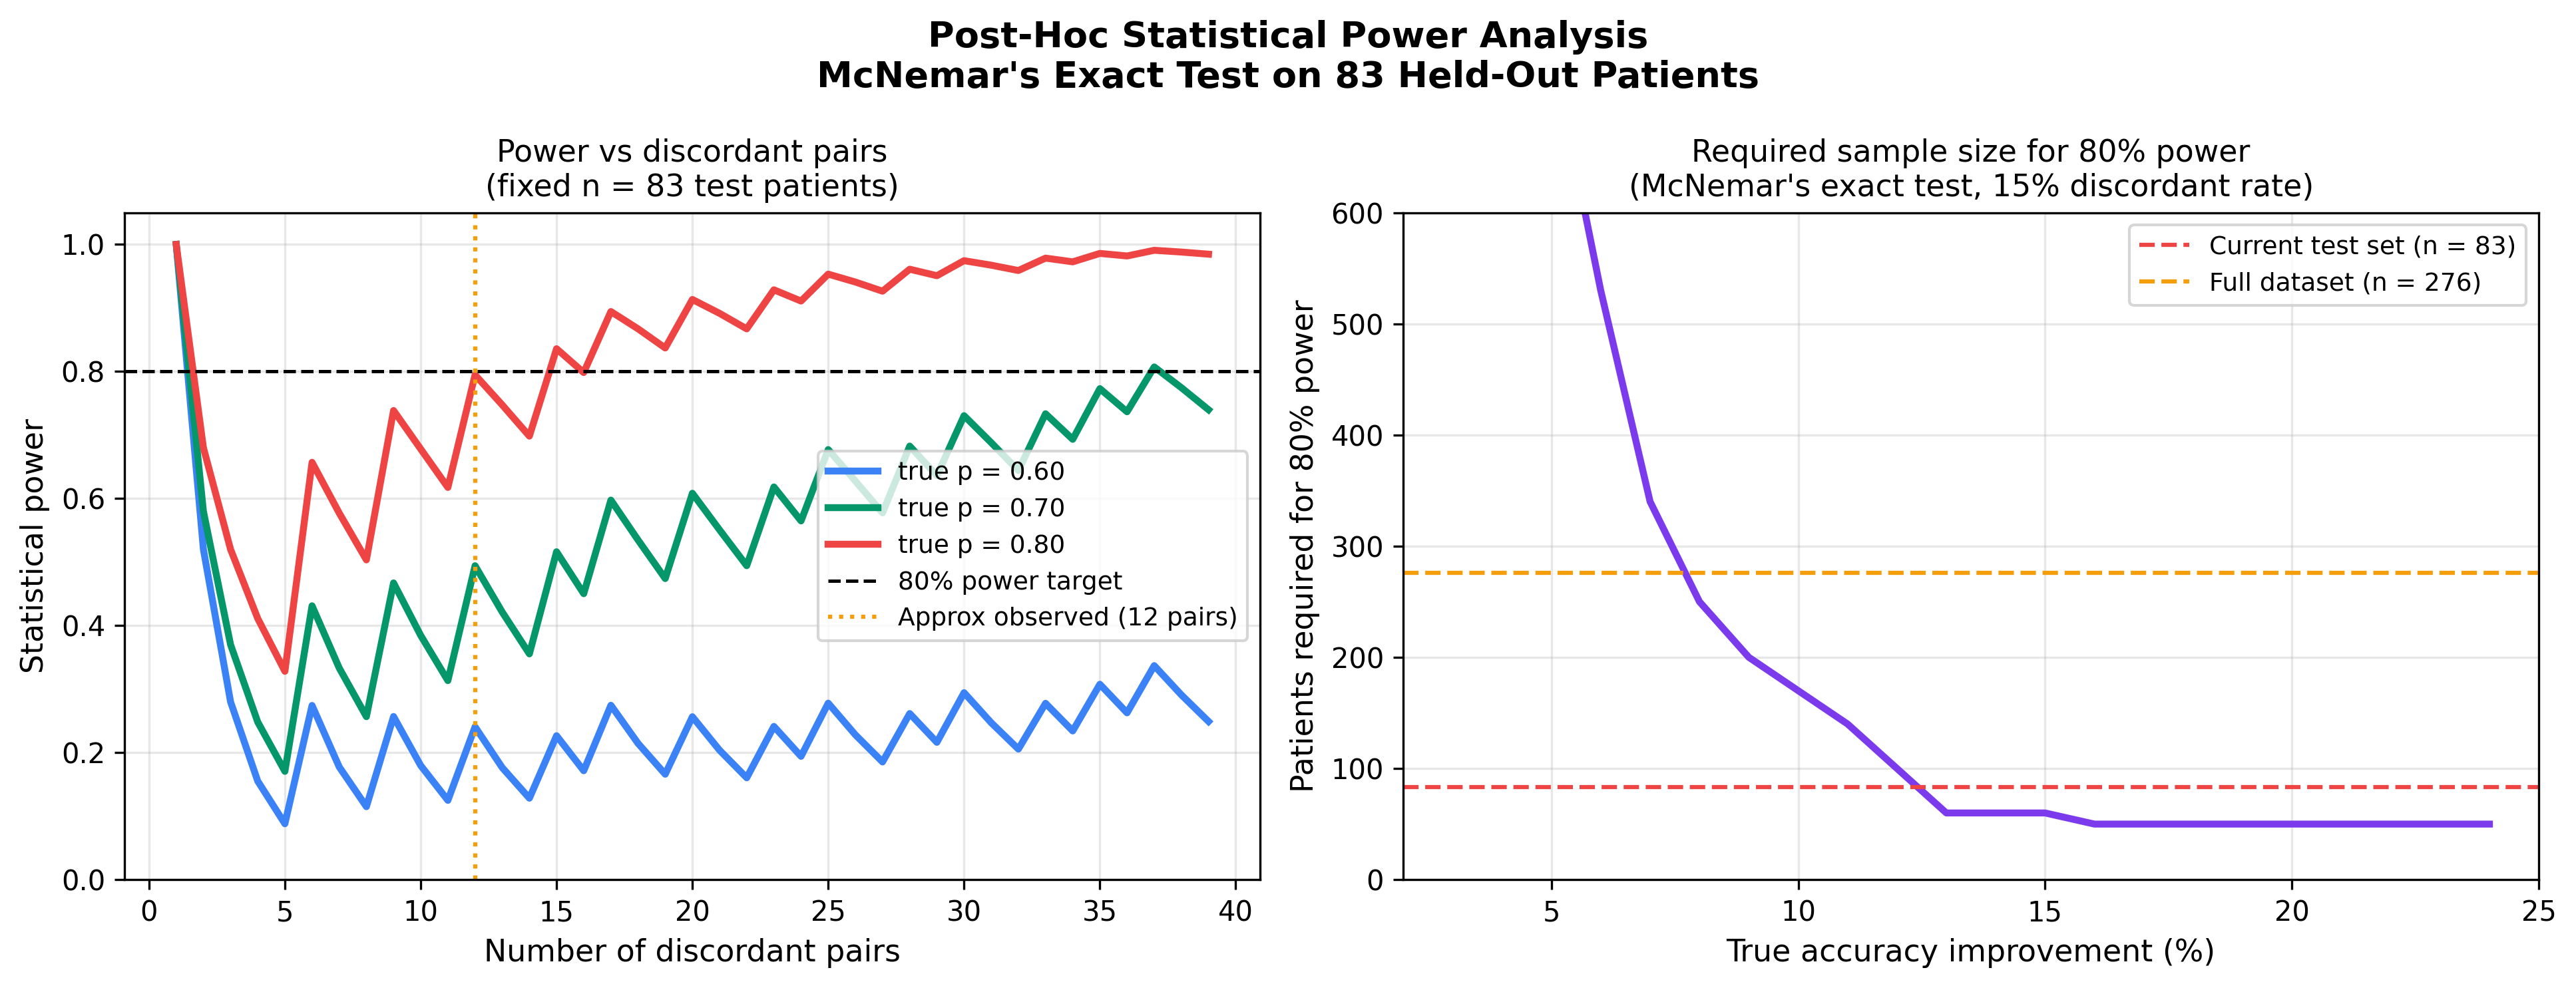
\includegraphics[width=\columnwidth]{power_analysis.png}
  \caption{Post-hoc power analysis for McNemar's exact test on 83 held-out patients. Left: statistical power as a function of discordant pair count for three true effect sizes. At 12 discordant pairs (the approximate observed rate), power does not reach 80\% for any effect size below true\_p~$= 0.80$. Right: required total patient count for 80\% power as a function of true accuracy improvement. Approximately 300 patients are needed for a moderate effect and over 550 for a small one. The dashed lines mark the current test set (83) and the full dataset (276).}
  \label{fig:power}
\end{figure}

An additional evaluation assessed whether a classifier trained exclusively on synthetic data can generalise to real patients. Using the 210 IQR-filtered CTGAN records as the sole training set and the held-out 83 real patients as the test set, Random Forest achieves AUC~$= 0.819$ and accuracy~$= 0.747$, Logistic Regression achieves AUC~$= 0.821$ and accuracy~$= 0.687$, and Gradient Boosting achieves AUC~$= 0.793$ and accuracy~$= 0.699$. These results demonstrate that classifiers trained entirely on synthetic CTGAN data retain a meaningful portion of their discriminative ability when tested on real patients, with AUC remaining above 0.79 for all three classifiers. This finding has direct relevance for federated IoMT settings where real patient data cannot be shared across institutions but synthetic surrogates are available: a model trained on synthetic data at a data-generating site can transfer meaningful predictive signal to a deployment site operating on real patients.

To partially address the single-dataset limitation, a subgroup consistency analysis was conducted across three clinically motivated splits of the 83-patient test set: disease stage (early: Stage 1--2, n~$= 17$; late: Stage 3--4, n~$= 66$), sex (female n~$= 72$; male n~$= 11$), and treatment arm (D-penicillamine n~$= 39$; placebo n~$= 44$). Classifiers trained under Scenario A and Scenario C were evaluated on each subgroup separately. Fig.~\ref{fig:subgroup} shows the results. For the three subgroups with at least 30 patients (late stage, female, and both treatment arms), AUC differences between Scenario A and Scenario C remained within $\pm 0.05$ across all three classifiers, and all AUC estimates exceeded 0.77. The null result is therefore directionally consistent across the primary clinical strata present in this cohort. The early-stage (n~$= 17$) and male (n~$= 11$) subgroups produced high-variance estimates that cannot support reliable inference; these are reported for transparency rather than as interpretable findings. External validation on an independent cohort remains necessary for a definitive generalisability claim.

\begin{figure}[t]
  \centering
  
\includegraphics[width=\columnwidth]{subgroup_analysis.png}
  \caption{Subgroup consistency analysis across three clinical splits of the 83-patient test set. Left: AUC by subgroup and classifier under Scenario A (real data only). Right: AUC under Scenario C (real plus equalised consensus). AUC differences between scenarios remain within $\pm 0.05$ for all subgroups with at least 30 patients. The dashed line marks the clinical usefulness threshold of AUC~$= 0.8$.}
  \label{fig:subgroup}
\end{figure}

To address the TVAE memorisation risk identified in the privacy analysis, a post-hoc output perturbation study was conducted. The filtered TVAE pool of 500 records has a near-duplicate rate of 38.2\% using the same 5th-percentile real-to-real distance threshold applied throughout the paper. Calibrated Gaussian noise was added to the eleven continuous features of each TVAE record after generation, with the noise scale expressed as a multiple of each feature's training-data standard deviation. At noise level $\sigma = 0.7$, the near-duplicate rate falls from 38.2\% to 2.8\%, while FID improves from 0.2194 to 0.0442, below the equalised consensus FID of 0.0862. The counterintuitive FID improvement arises because the TVAE, with its lower FID in some dimensions, was nevertheless generating records clustered near specific real patients; dispersing those clusters moves the marginal distributions closer to the real training distribution. Fig.~\ref{fig:privacy_enh} shows the full noise--privacy and noise--quality tradeoff curves alongside estimated DP-SGD privacy budgets. Moments-accountant estimates across noise multiplier values from 0.5 to 3.0 produce epsilon values between 14.0 and 210.4 at $\delta = 10^{-5}$, all in the range classified as providing no practical differential privacy guarantee. This finding confirms that formal DP-SGD training is not feasible at $n = 193$ training patients: at any noise level that would provide a meaningful epsilon ($\varepsilon \leq 3$), the gradient noise would destroy the latent structure needed for coherent synthetic data generation. Output perturbation at $\sigma = 0.7$ is therefore presented as an effective post-hoc privacy mitigation for the TVAE pool, reducing the near-duplicate rate to below 3\% with a simultaneous improvement in distributional fidelity. Retraining with formal DP-SGD objectives on a larger cohort of at least several hundred patients remains the recommended direction for deployments where formal privacy guarantees are required.

\begin{figure}[t]
  \centering
  
\includegraphics[width=\columnwidth]{privacy_enhancement.png}
  \caption{TVAE privacy enhancement analysis. Left: near-duplicate rate versus output noise level $\sigma$ in units of feature standard deviation. At $\sigma = 0.7$, the near-duplicate rate falls from 38.2\% to 2.8\%. Centre: FID score versus noise level; FID improves from 0.2194 to 0.0442 at $\sigma = 0.7$, indicating that dispersing memorised clusters improves distributional alignment. Right: DP-SGD epsilon estimates across noise multiplier values. All estimated epsilon values exceed 14, confirming that formal differential privacy is impractical at $n = 193$ training patients and should be deferred to larger-cohort replications.}
  \label{fig:privacy_enh}
\end{figure}

Fig.~\ref{fig:importance} shows feature importance rankings from Random Forest and Gradient Boosting trained under Scenario A. Both classifiers consistently rank continuous laboratory biomarkers highest, with N\_Days and Bilirubin leading across both methods, followed by Prothrombin and Albumin. Binary clinical indicators such as Ascites, Drug, Spiders, and Edema carry comparatively low weight. This pattern is clinically coherent and validates the integrity of the preprocessing and modelling pipeline.

\begin{figure}[t]
  \centering
  
\includegraphics[width=\columnwidth]{feature_importance.png}
  \caption{Feature importance rankings from Random Forest (left) and Gradient Boosting (right) trained on real data only under Scenario A. Both classifiers consistently rank continuous laboratory biomarkers highest. N\_Days and Bilirubin are the two leading predictors across both classifiers, followed by Prothrombin and Albumin. Binary clinical indicators show comparatively low importance, consistent with the dominant role of laboratory measurements in PBC prognosis.}
  \label{fig:importance}
\end{figure}

% ---------------------------------------------------------------
% Section V: Conclusion
% ---------------------------------------------------------------
\FloatBarrier
\section{Conclusion}
\label{sec:conclusion}

This study investigated whether deep generative synthetic data augmentation can improve liver cirrhosis survival prediction in an IoMT setting, using the Mayo Clinic PBC dataset as a controlled rare-disease tabular data scenario. Three generative architectures were trained from scratch and evaluated through a pipeline that goes beyond distributional fidelity to directly measure predictive utility on real held-out patients.

Two methodological contributions were introduced. An IQR-based physiological plausibility filter removes synthetic records with clinically implausible biomarker values before any downstream use, discarding between 54 and 58 per cent of adversarially generated records. A multi-method consensus voting mechanism accepts only synthetic patients corroborated independently by all three generative architectures in a standardised feature space.

Four empirical findings stand out. Among individual generative models, CTGAN produces the best distributional fidelity at FID~$= 0.075$ and the most acceptable privacy profile at 9.0 per cent near-duplicates, making it the most suitable model for privacy-constrained IoMT augmentation. On the 83-patient held-out test set, no augmentation scenario achieves a statistically significant improvement over the real-data baseline, confirming that distributional similarity does not guarantee predictive gain on real patients. Consensus augmentation reduces Gradient Boosting cross-validation AUC variance 4.9-fold (from 0.069 to 0.014) and Random Forest variance 3.4-fold (from 0.053 to 0.016), demonstrating that synthetic patients drawn from a cross-architecture agreement region stabilise classifiers in a way that random oversampling methods do not. An additional synthetic-only evaluation shows that classifiers trained exclusively on 210 CTGAN-generated records and tested on 83 real patients achieve AUC values between 0.793 and 0.821, demonstrating that synthetic data retains transferable predictive signal even without any real patient exposure during training.

A post-hoc power analysis shows that McNemar's exact test on 83 patients carries only 9\% power to detect a genuine 5 percentage-point accuracy gain; approximately 300 patients would be required for 80\% power at that effect size. A post-hoc output perturbation analysis demonstrates that adding Gaussian noise at $\sigma = 0.7$ feature standard deviations to TVAE-generated records reduces the near-duplicate rate from 38.2\% to 2.8\% while simultaneously improving TVAE FID from 0.2194 to 0.0442, providing a practical post-hoc privacy mitigation without model retraining. Formal DP-SGD training remains impractical at $n = 193$ (estimated $\varepsilon > 14$ across all evaluated noise levels). Future work should examine the stability effect on larger cohorts and external validation sites, and should investigate DP-TVAE training once a dataset of several hundred patients is available. Extending the framework to longitudinal IoMT data streams, where temporal dependencies introduce additional generation challenges beyond those present in single-visit tabular records, represents a further natural direction for this line of research.

% ---------------------------------------------------------------
% References
% ---------------------------------------------------------------
\begin{thebibliography}{99}

\bibitem{guo2021}
A. Guo, N.~R. Mazumder, D.~P. Ladner, and R.~E. Foraker, ``Predicting mortality among patients with liver cirrhosis in electronic health records with machine learning,'' \textit{PLoS ONE}, vol.~16, no.~8, p.~e0256428, Aug.~2021, doi:~10.1371/journal.pone.0256428.

\bibitem{obeid2023}
J.~S. Obeid, A. Khalifa, B. Xavier, H. Bou-Daher, and D.~C. Rockey, ``An AI approach for identifying patients with cirrhosis,'' \textit{J. Clin. Gastroenterol.}, vol.~57, no.~1, pp.~82--88, Jul.~2021, doi:~10.1097/mcg.0000000000001586.

\bibitem{kanwal2020}
F. Kanwal \textit{et al.}, ``Development, validation, and evaluation of a simple machine learning model to predict cirrhosis mortality,'' \textit{JAMA Netw. Open}, vol.~3, no.~11, p.~e2023780, Nov.~2020, doi:~10.1001/jamanetworkopen.2020.23780.

\bibitem{goncalves2020}
A. Goncalves, P. Ray, B. Soper, J. Stevens, L. Coyle, and A.~P. Sales, ``Generation and evaluation of synthetic patient data,'' \textit{BMC Med. Res. Methodol.}, vol.~20, no.~1, p.~108, May~2020, doi:~10.1186/s12874-020-00977-1.

\bibitem{gonzales2023}
A. Gonzales, G. Guruswamy, and S.~R. Smith, ``Synthetic data in health care: A narrative review,'' \textit{PLoS Digit. Health}, vol.~2, no.~1, p.~e0000082, Jan.~2023, doi:~10.1371/journal.pdig.0000082.

\bibitem{yan2022}
C. Yan \textit{et al.}, ``A multifaceted benchmarking of synthetic electronic health record generation models,'' \textit{Nat. Commun.}, vol.~13, no.~1, p.~7609, Dec.~2022, doi:~10.1038/s41467-022-35295-1.

\bibitem{nikolentzos2023}
G. Nikolentzos, M. Vazirgiannis, C. Xypolopoulos, M. Lingman, and E.~G. Brandt, ``Synthetic electronic health records generated with variational graph autoencoders,'' \textit{NPJ Digit. Med.}, vol.~6, no.~1, p.~83, Apr.~2023, doi:~10.1038/s41746-023-00822-x.

\bibitem{che2017}
Z. Che, Y. Cheng, S. Zhai, Z. Sun, and Y. Liu, ``Boosting deep learning risk prediction with generative adversarial networks for electronic health records,'' in \textit{Proc. IEEE Int. Conf. Data Min.}, 2017, pp.~787--792, doi:~10.1109/icdm.2017.93.

\bibitem{kababji2023}
S.~E. Kababji \textit{et al.}, ``Evaluating the utility and privacy of synthetic breast cancer clinical trial data sets,'' \textit{JCO Clin. Cancer Inform.}, no.~7, p.~e2300116, Sep.~2023, doi:~10.1200/cci.23.00116.

\bibitem{espinosa2023}
E. Espinosa and A. Figueira, ``On the quality of synthetic generated tabular data,'' \textit{Mathematics}, vol.~11, no.~15, p.~3278, Jul.~2023, doi:~10.3390/math11153278.

\bibitem{guillaudeux2023}
M. Guillaudeux \textit{et al.}, ``Patient-centric synthetic data generation, no reason to risk re-identification in biomedical data analysis,'' \textit{NPJ Digit. Med.}, vol.~6, no.~1, p.~37, Mar.~2023, doi:~10.1038/s41746-023-00771-5.

\bibitem{kumari2024}
C. Kumari and R. Siddharthan, ``MMM and MMMSynth: Clustering of heterogeneous tabular data, and synthetic data generation,'' \textit{PLoS ONE}, vol.~19, no.~4, p.~e0302271, Apr.~2024, doi:~10.1371/journal.pone.0302271.

\bibitem{figueira2022}
A. Figueira and B. Vaz, ``Survey on synthetic data generation, evaluation methods and GANs,'' \textit{Mathematics}, vol.~10, no.~15, p.~2733, Aug.~2022, doi:~10.3390/math10152733.

\bibitem{vega2020}
B. Vega-M\'{a}rquez, C. Rubio-Escudero, and I. Nepomuceno-Chamorro, ``Generation of synthetic data with conditional generative adversarial networks,'' \textit{Log. J. IGPL}, vol.~30, no.~2, pp.~252--262, Nov.~2020, doi:~10.1093/jigpal/jzaa059.

\bibitem{choi2017}
E. Choi, S. Biswal, B. Malin, J. Duke, W.~F. Stewart, and J. Sun, ``Generating multi-label discrete patient records using generative adversarial networks,'' \textit{arXiv}, Mar.~2017, doi:~10.48550/arxiv.1703.06490.

\bibitem{lenz2021}
S. Lenz, M. Hess, and H. Binder, ``Deep generative models in DataSHIELD,'' \textit{BMC Med. Res. Methodol.}, vol.~21, no.~1, p.~64, Apr.~2021, doi:~10.1186/s12874-021-01237-6.

\bibitem{sharma2024}
D. Sharma, W. Lou, and W. Xu, ``PhylaGAN: Data augmentation through conditional GANs and autoencoders for improving disease prediction accuracy using microbiome data,'' \textit{Bioinformatics}, vol.~40, no.~4, p.~btae161, Apr.~2024, doi:~10.1093/bioinformatics/btae161.

\bibitem{meidan2018}
Y. Meidan \textit{et al.}, ``N-BaIoT: Network-based detection of IoT botnet attacks using deep autoencoders,'' \textit{IEEE Pervasive Comput.}, vol.~17, no.~3, pp.~12--22, Jul.~2018, doi:~10.1109/mprv.2018.03367731.

\bibitem{damico2023}
S. D'Amico \textit{et al.}, ``Synthetic data generation by artificial intelligence to accelerate research and precision medicine in hematology,'' \textit{JCO Clin. Cancer Inform.}, no.~7, p.~e2300021, Jun.~2023, doi:~10.1200/cci.23.00021.

\bibitem{kim2024}
H. Kim \textit{et al.}, ``Synthetic data improve survival status prediction models in early-onset colorectal cancer,'' \textit{JCO Clin. Cancer Inform.}, no.~8, p.~e2300201, Jan.~2024, doi:~10.1200/cci.23.00201.

\bibitem{tucker2020}
A. Tucker, Z. Wang, Y. Rotalinti, and P. Myles, ``Generating high-fidelity synthetic patient data for assessing machine learning healthcare software,'' \textit{NPJ Digit. Med.}, vol.~3, no.~1, p.~147, Nov.~2020, doi:~10.1038/s41746-020-00353-9.

\bibitem{dankar2022}
F.~K. Dankar, M.~K. Ibrahim, and L. Ismail, ``A multi-dimensional evaluation of synthetic data generators,'' \textit{IEEE Access}, vol.~10, pp.~11147--11158, Jan.~2022, doi:~10.1109/access.2022.3144765.

\bibitem{foraker2020}
R.~E. Foraker \textit{et al.}, ``Spot the difference: Comparing results of analyses from real patient data and synthetic derivatives,'' \textit{JAMIA Open}, vol.~3, no.~4, pp.~557--566, Dec.~2020, doi:~10.1093/jamiaopen/ooaa060.

\bibitem{kaabachi2023}
B. Kaabachi \textit{et al.}, ``A scoping review of privacy and utility metrics in medical synthetic data,'' \textit{medRxiv}, Nov.~2023, doi:~10.1101/2023.11.28.23299124.

\bibitem{jiang2023}
X. Jiang, J. Zheng, X. Zhuang, and Z. Ge, ``Ensemble data augmentation for imbalanced fault diagnosis,'' \textit{IEEE Trans. Instrum. Meas.}, vol.~72, pp.~1--12, Jan.~2023, doi:~10.1109/tim.2023.3307757.

\bibitem{pandey2025}
C. Pandey, V. Tiwari, S.~A.~J. Francis, V. Pal, and D.~S. Roy, ``MF-CGAN: Multifeature conditional GAN for synthetic data generation in Internet of Medical Things,'' \textit{IEEE Internet Things J.}, vol.~12, no.~10, pp.~13469--13476, Mar.~2025, doi:~10.1109/jiot.2025.3554207.

\end{thebibliography}

\end{document}
